% !TEX root = ../my-thesis.tex
\chapter{Ergänzende Grafiken}
\label{app:grafiken}

\section{Laufartefakte in Nextflow}
\label{app:grafiken:nextflow}

\begin{figure}[ht]
  \centering
  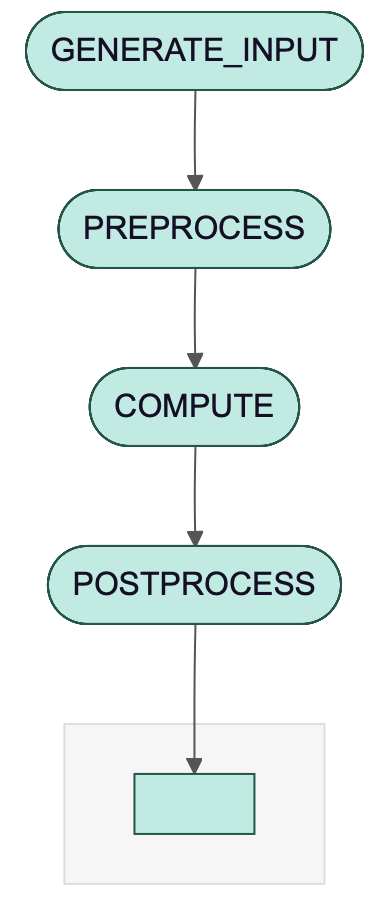
\includegraphics[width=0.30\textwidth,height=0.32\textheight,keepaspectratio]{content/figs/nextflow/nextflow_dag_pl}
  \caption{Von Nextflow erzeugter Workflow-Graph des Pipeline-Workflows}
  \label{fig:nf:dag}
\end{figure}

\begin{figure}[ht]
  \centering
  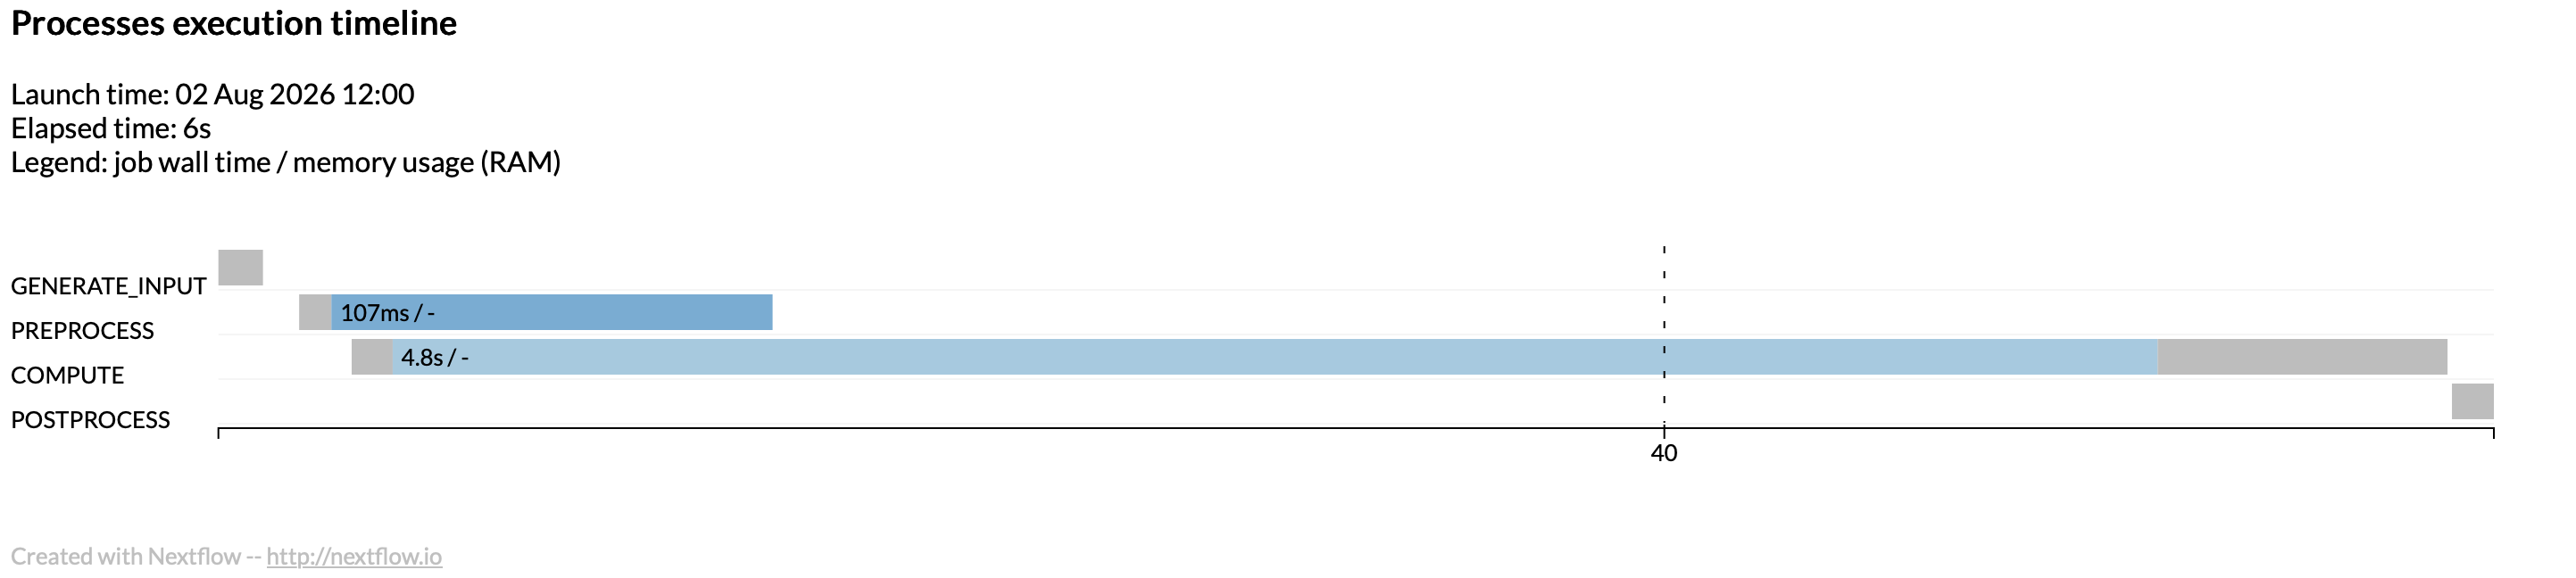
\includegraphics[width=0.92\textwidth,height=0.26\textheight,keepaspectratio]{content/figs/nextflow/nextflow_timeline_pipeline_short}
  \caption[Zeitstrahl eines Pipeline-Laufs mit der kurzen Rechenlast]{Zeitstrahl eines Pipeline-Laufs mit der kurzen Rechenlast. Die Balken von REPROCESS wurde auf eine Mindestbreite von circa einer Sekunde gezogen. Der Schritt \texttt{PREPROCESS} dauerte laut Bericht 102\,ms, sein Balken erscheint dadurch rund zehnmal zu lang und ragt über den Beginn von \texttt{COMPUTE} hinaus. Die Ausführungszeiten überschneiden sich tatsächlich nicht.}
  \label{fig:nf:timeline:short}
\end{figure}

\begin{figure}[ht]
  \centering
  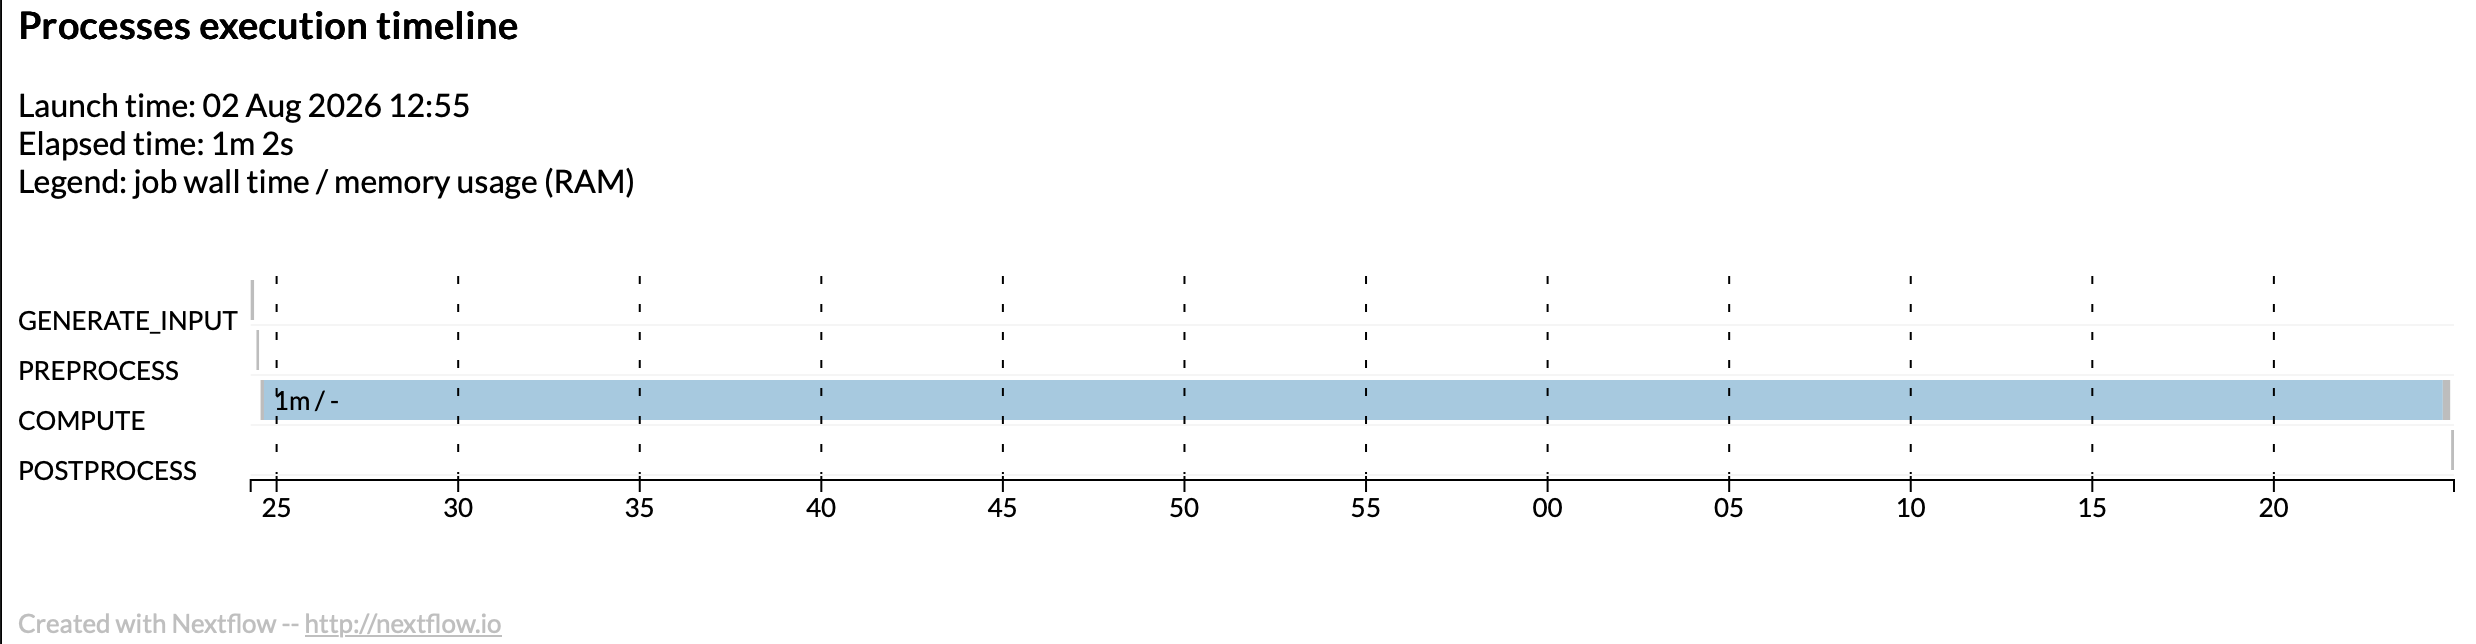
\includegraphics[width=0.92\textwidth,height=0.26\textheight,keepaspectratio]{content/figs/nextflow/nextflow_timeline_pipeline_medium}
  \caption{Von Nextflow erzeugter Zeitstrahl eines Pipeline-Laufs mit der mittleren Rechenlast}
  \label{fig:nf:timeline}
\end{figure}

\begin{figure}[ht]
  \centering
  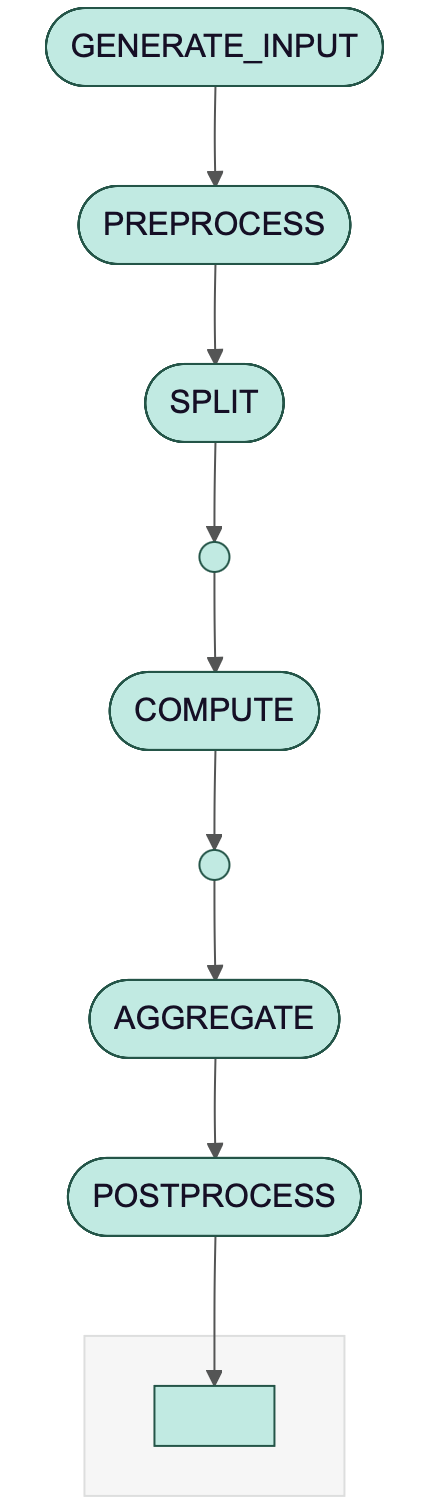
\includegraphics[width=0.30\textwidth,height=0.32\textheight,keepaspectratio]{content/figs/nextflow/nextflow_dag_sg}
  \caption{Von Nextflow erzeugter Workflow-Graph des Scatter-Gather-Workflows}
  \label{fig:nf:dag:sg}
\end{figure}

\begin{figure}[ht]
  \centering
  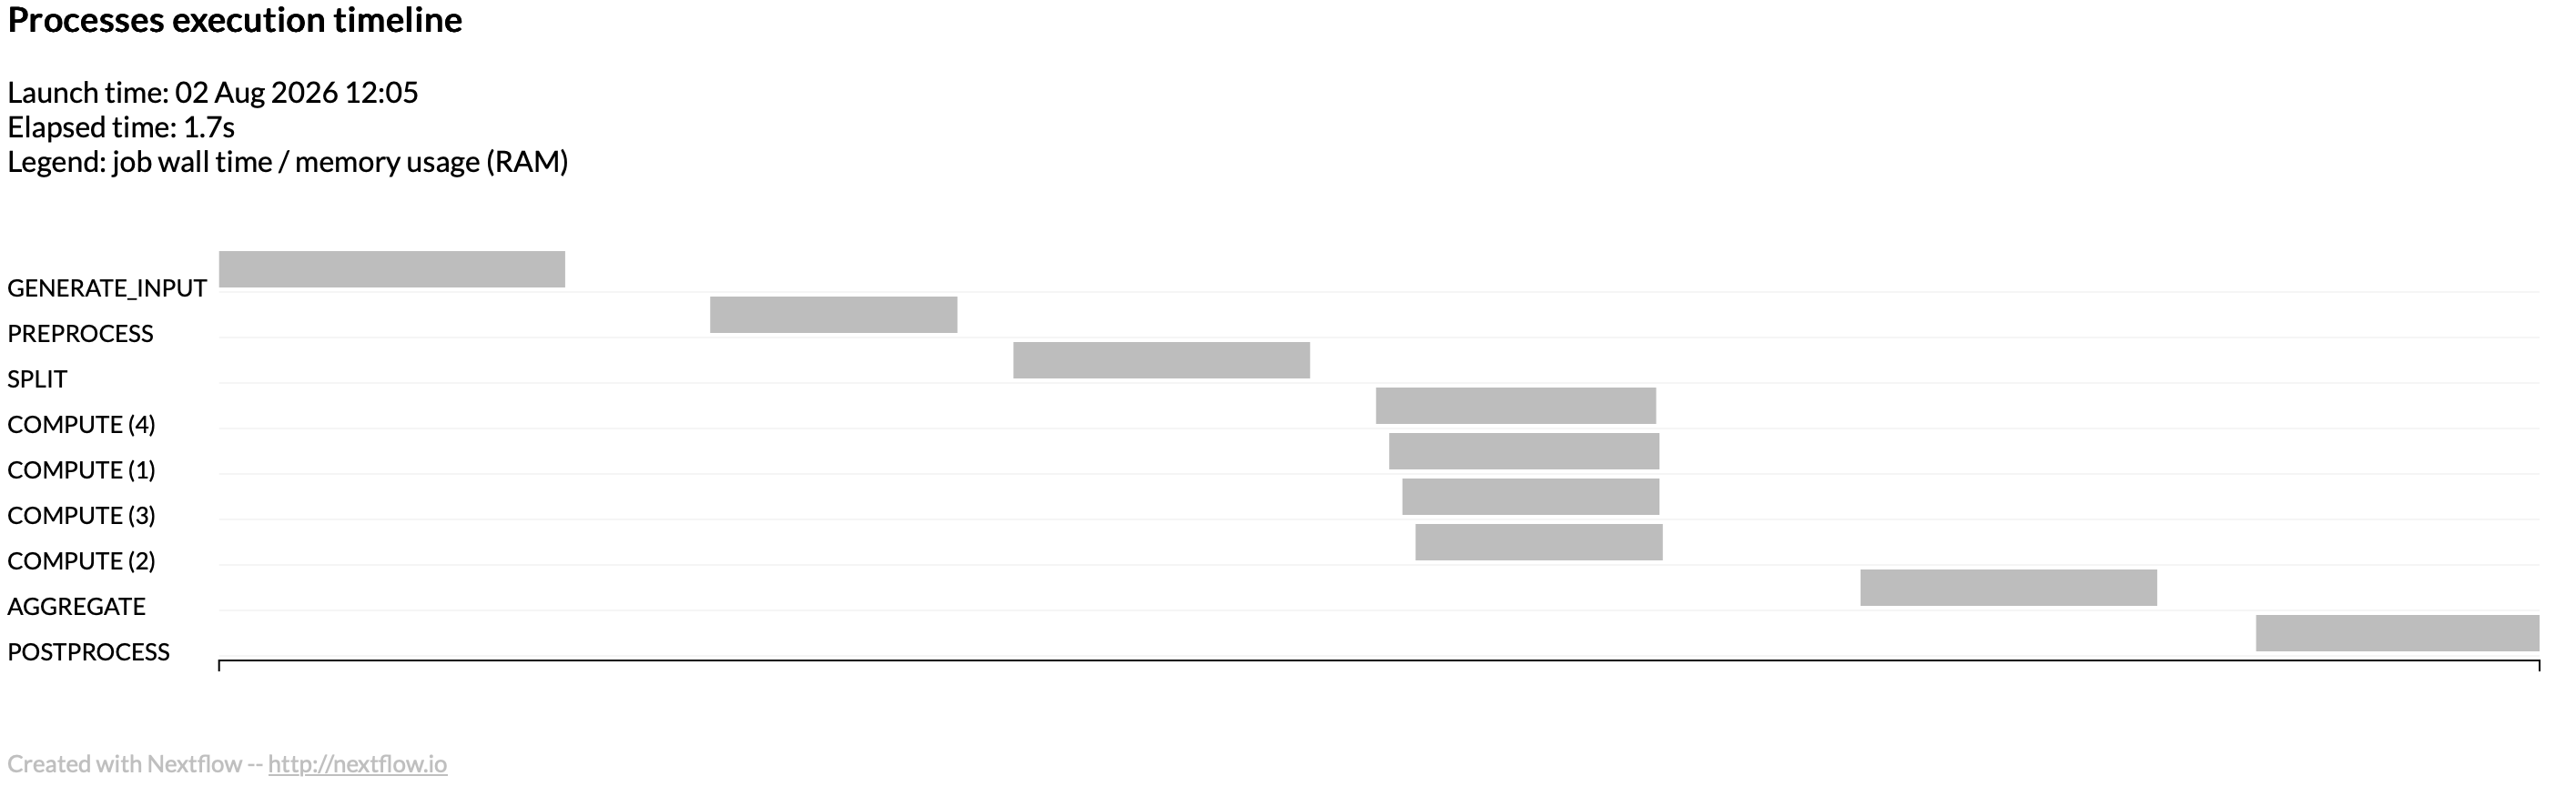
\includegraphics[width=0.92\textwidth,height=0.26\textheight,keepaspectratio]{content/figs/nextflow/nextflow_timeline_sg_short}
  \caption{Von Nextflow erzeugter Zeitstrahl eines Scatter-Gather-Laufs mit vier Teilstücken und kurzer Rechenlast}
  \label{fig:nf:timeline:sg}
\end{figure}

\FloatBarrier
\section{Laufartefakte in StreamFlow}
\label{app:grafiken:streamflow}

\begin{figure}[ht]
  \centering
  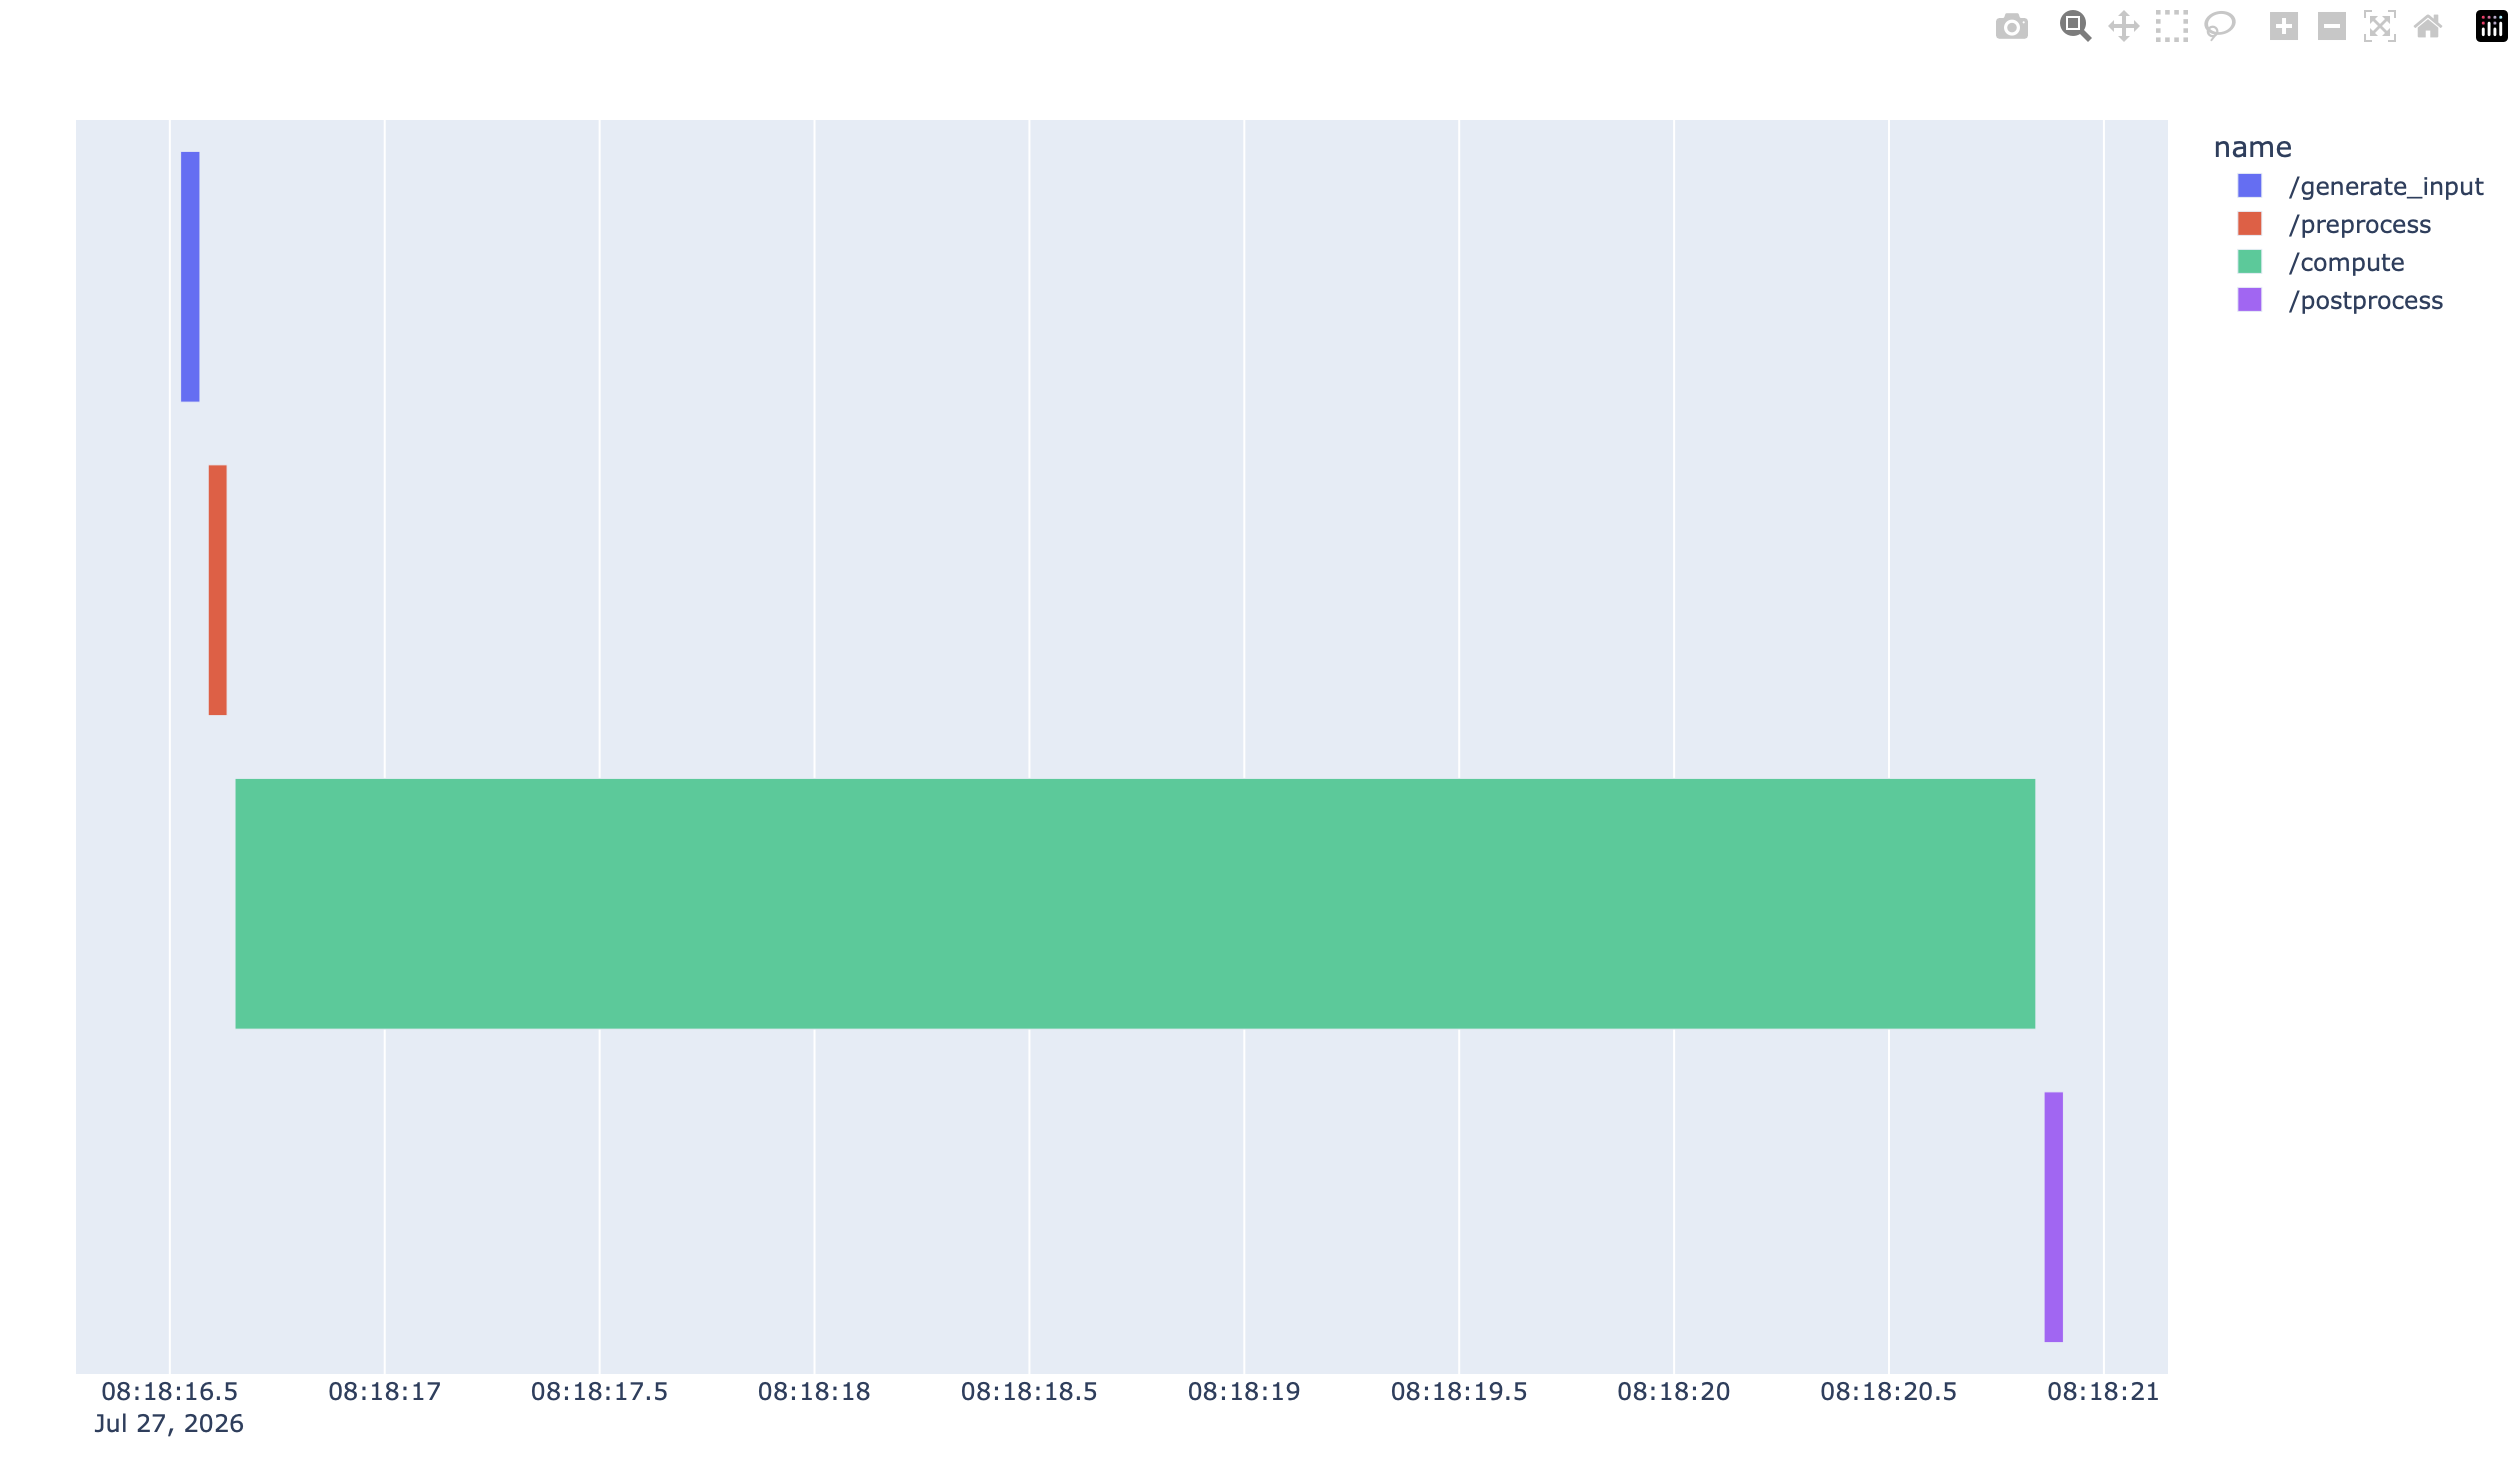
\includegraphics[width=0.92\textwidth,height=0.26\textheight,keepaspectratio]{content/figs/streamflow/streamflow_pipeline_timeline}
  \caption{Von StreamFlow erzeugter Zeitstrahl eines Pipeline-Laufs mit der kurzen Rechenlast}
  \label{fig:sf:timeline}
\end{figure}

\begin{figure}[ht]
  \centering
  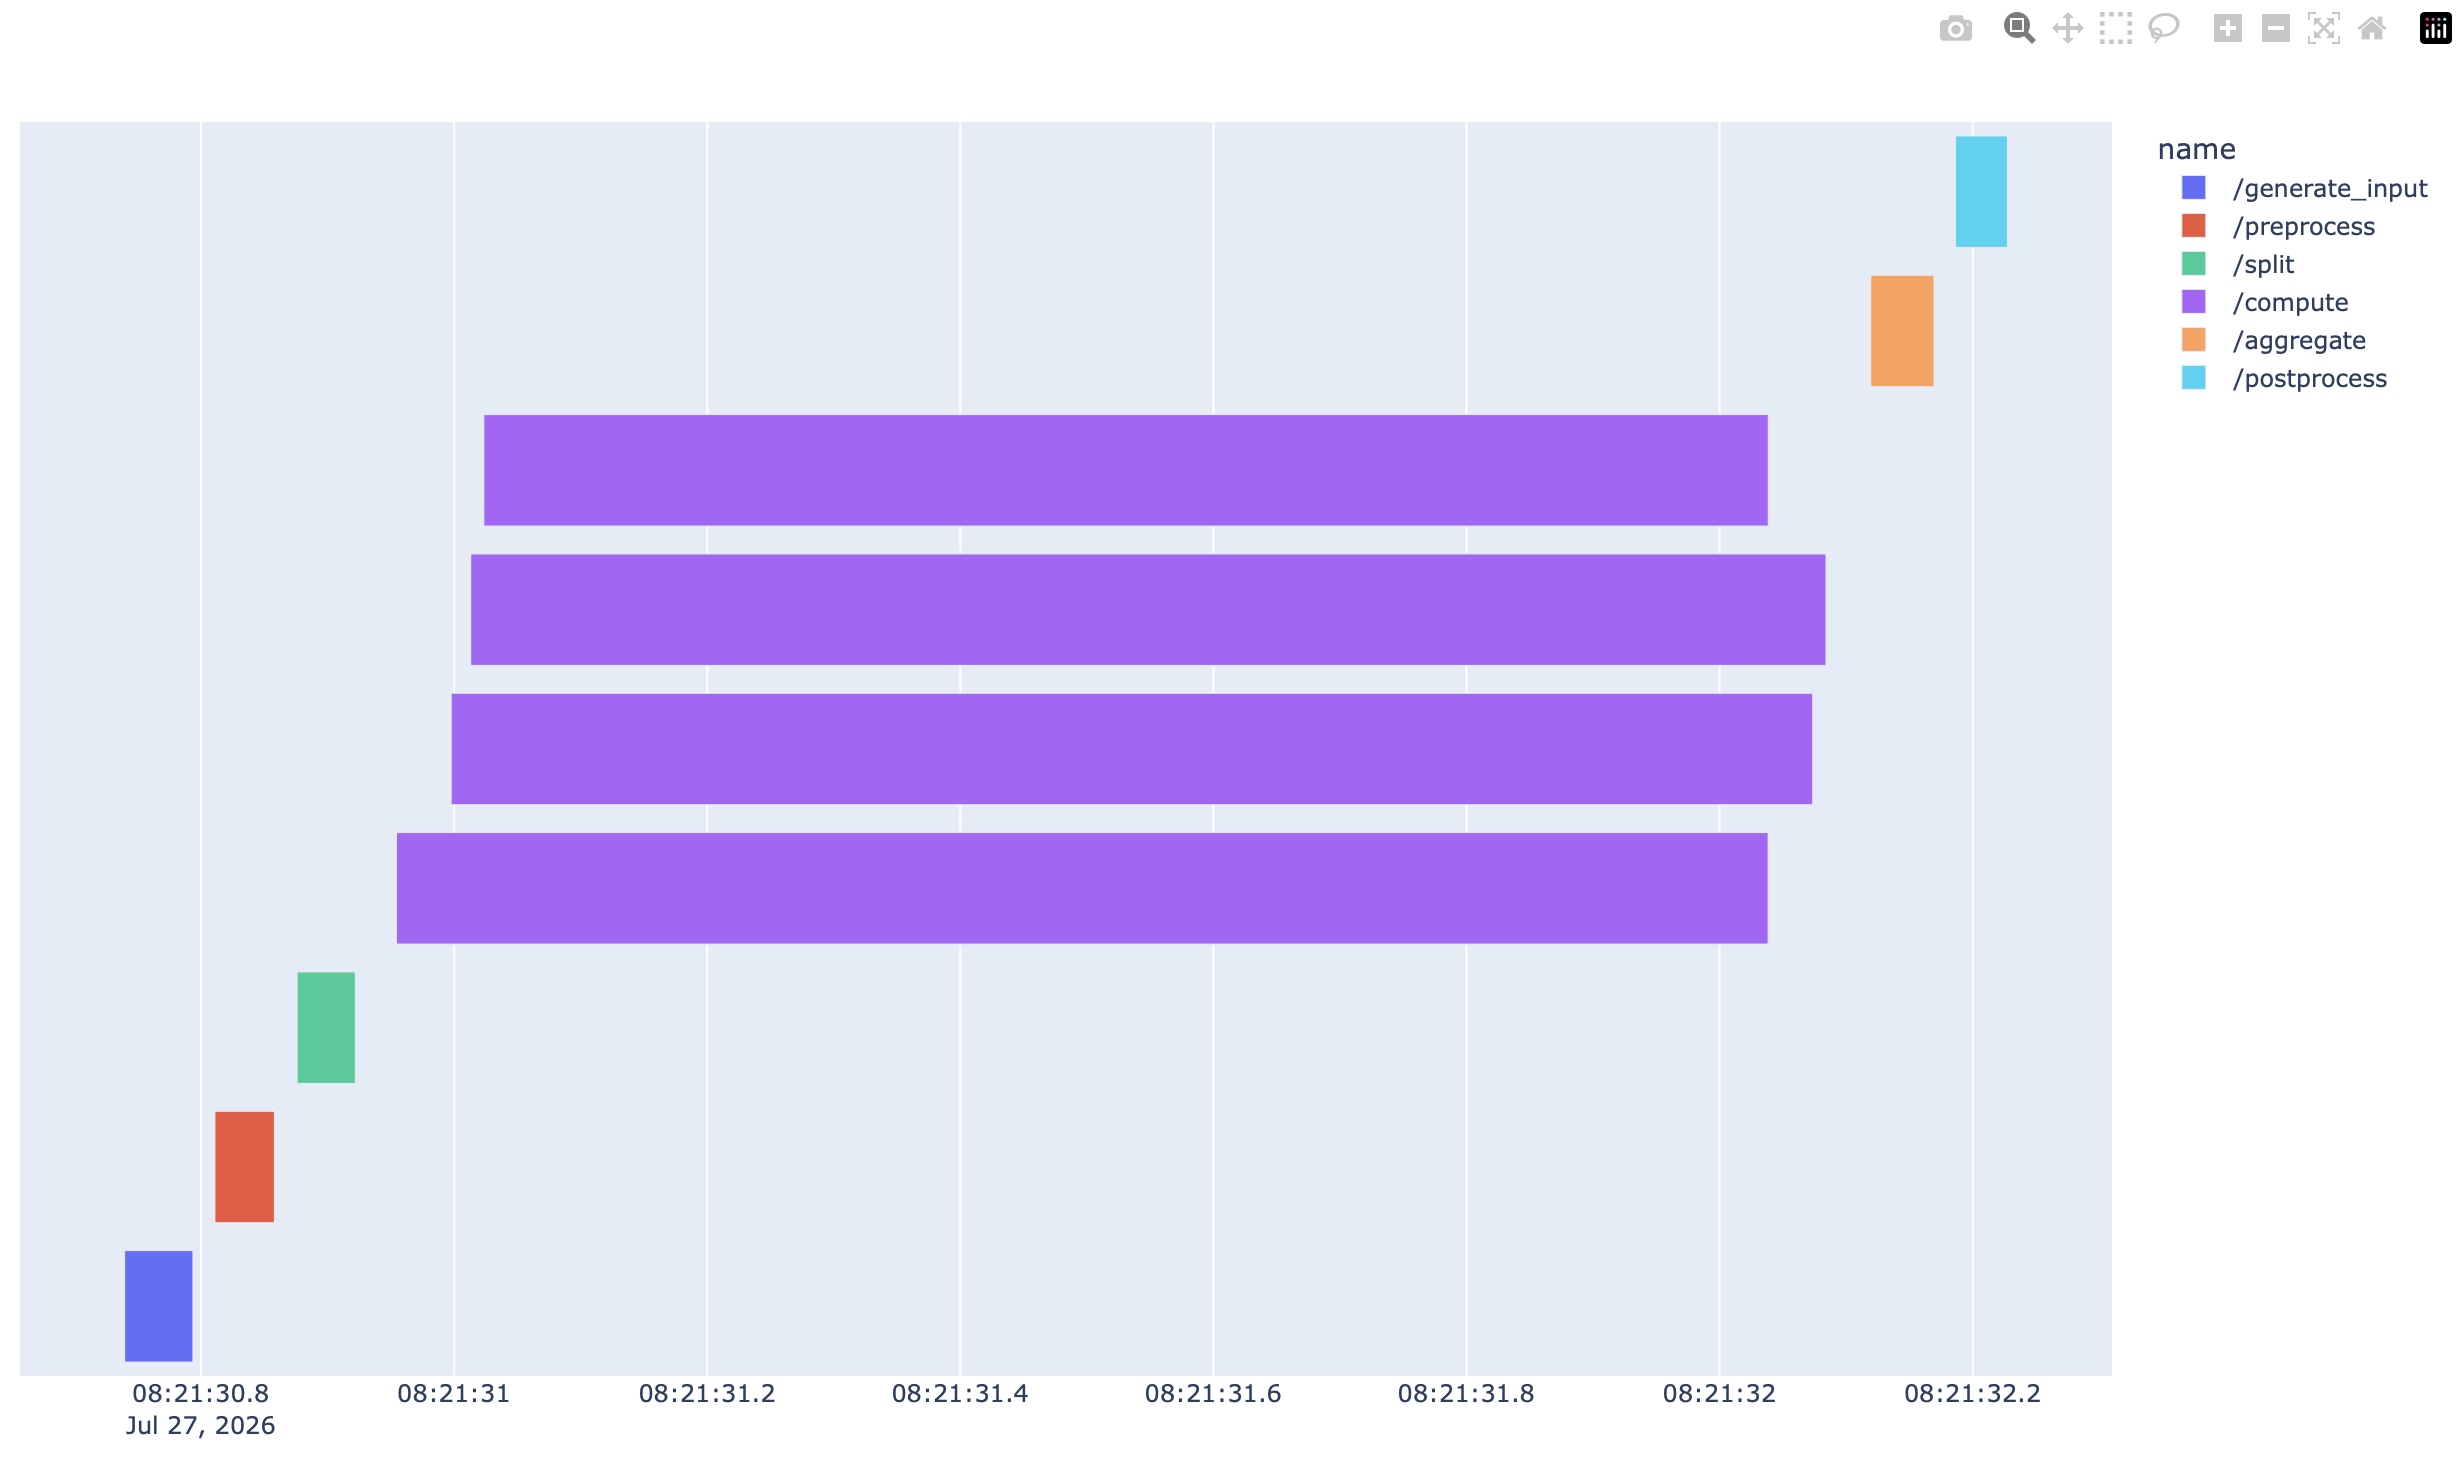
\includegraphics[width=0.92\textwidth,height=0.26\textheight,keepaspectratio]{content/figs/streamflow/streamflow_sg_timeline}
  \caption{Von StreamFlow erzeugter Zeitstrahl eines Scatter-Gather-Laufs}
  \label{fig:sf:timeline:sg}
\end{figure}

\FloatBarrier
\section{Laufartefakte in Pegasus}
\label{app:grafiken:pegasus}

\begin{figure}[ht]
  \centering
  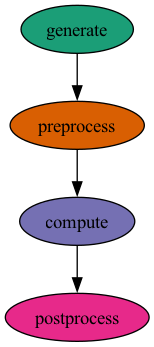
\includegraphics[width=0.42\textwidth,height=0.30\textheight,keepaspectratio]{content/figs/pegasus/pegasus-pipeline-benchmark-0-abstract}
  \caption{Von Pegasus erzeugte abstrakte Darstellung des Pipeline-Workflows}
  \label{fig:pg:dag}
\end{figure}

\begin{figure}[ht]
  \centering
  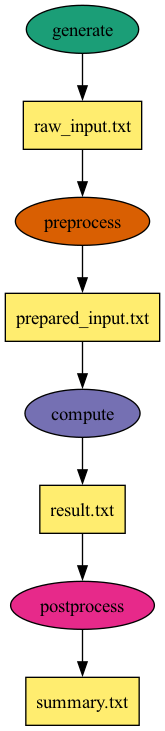
\includegraphics[width=0.42\textwidth,height=0.30\textheight,keepaspectratio]{content/figs/pegasus/pegasus-pipeline-benchmark-0-abstract-files}
  \caption{Von Pegasus erzeugte Darstellung des Pipeline-Workflows mit den beteiligten Dateien}
  \label{fig:pg:dag:files}
\end{figure}

\begin{figure}[ht]
  \centering
  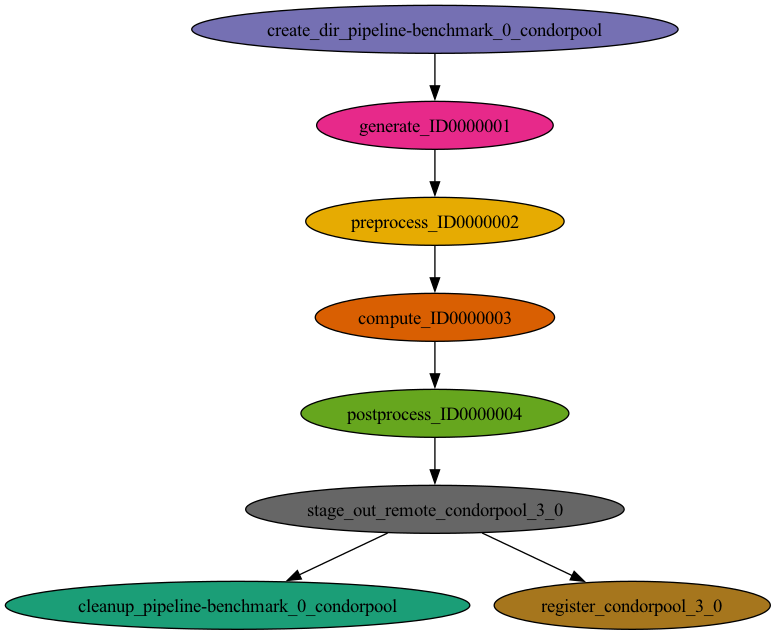
\includegraphics[width=0.42\textwidth,height=0.30\textheight,keepaspectratio]{content/figs/pegasus/pegasus-pipeline-benchmark-0-concrete}
  \caption{Von Pegasus erzeugte Darstellung des geplanten Graphen desselben Workflows}
  \label{fig:pg:dag:concrete}
\end{figure}

\begin{figure}[ht]
  \centering
  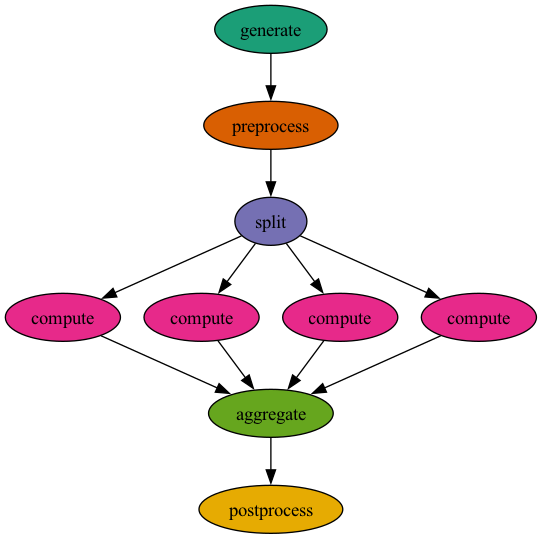
\includegraphics[width=0.42\textwidth,height=0.30\textheight,keepaspectratio]{content/figs/pegasus/scatter-gather-benchmark-0-abstract}
  \caption{Von Pegasus erzeugte abstrakte Darstellung des Scatter-Gather-Workflows mit vier Teilstücken}
  \label{fig:pg:dag:sg}
\end{figure}

\begin{figure}[ht]
  \centering
  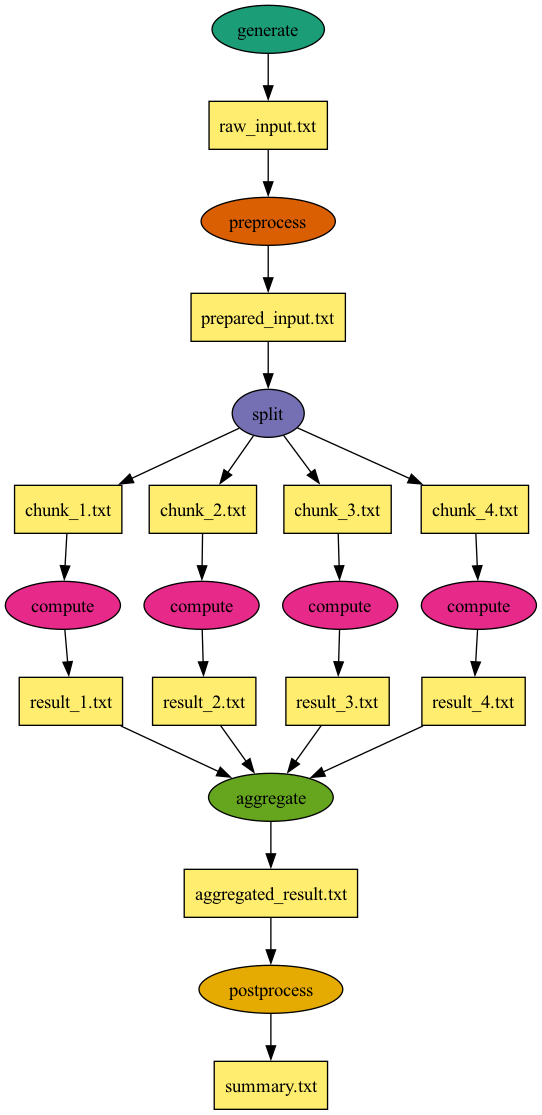
\includegraphics[width=0.42\textwidth,height=0.30\textheight,keepaspectratio]{content/figs/pegasus/scatter-gather-benchmark-0-abstract-files}
  \caption{Von Pegasus erzeugte Darstellung des Scatter-Gather-Workflows mit den beteiligten Dateien}
  \label{fig:pg:dag:sg:files}
\end{figure}

\begin{figure}[ht]
  \centering
  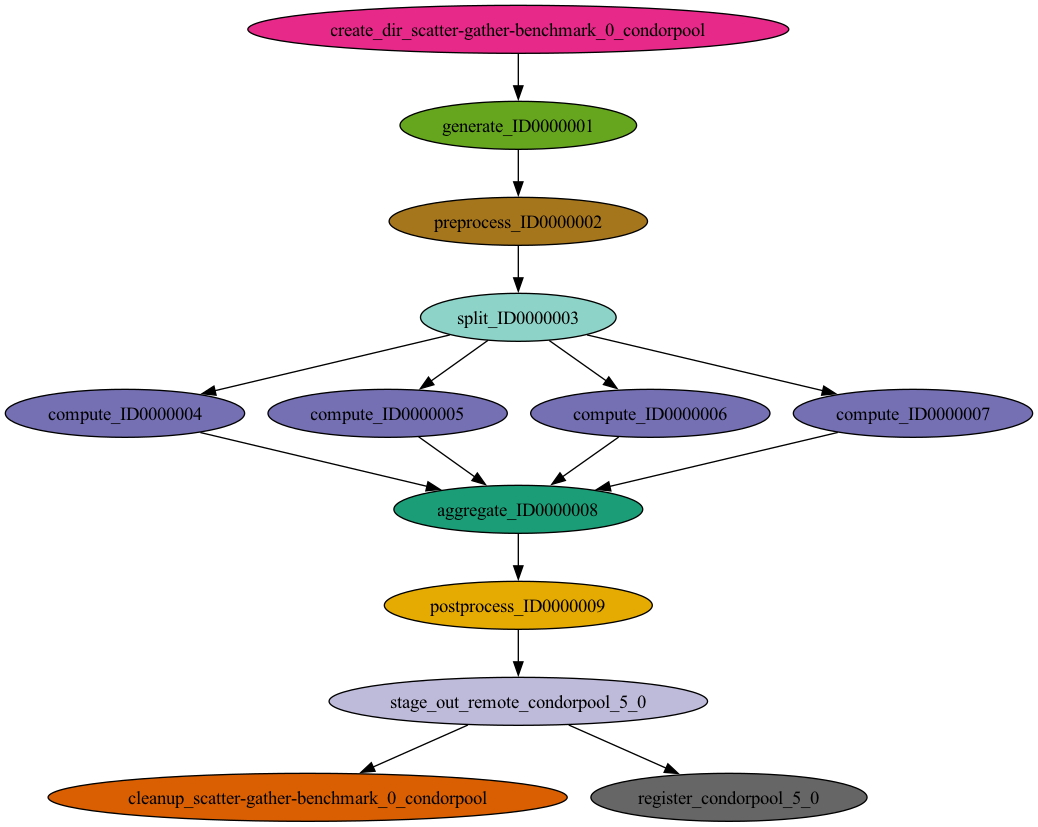
\includegraphics[width=0.42\textwidth,height=0.30\textheight,keepaspectratio]{content/figs/pegasus/scatter-gather-benchmark-0-concrete}
  \caption{Von Pegasus erzeugte Darstellung des geplanten Graphen desselben Workflows}
  \label{fig:pg:dag:sg:concrete}
\end{figure}

\FloatBarrier
\clearpage
\section{Laufartefakte in AiiDA}
\label{app:grafiken:aiida}
\vspace*{-0.6\baselineskip}

\begin{figure}[H]
  \centering
  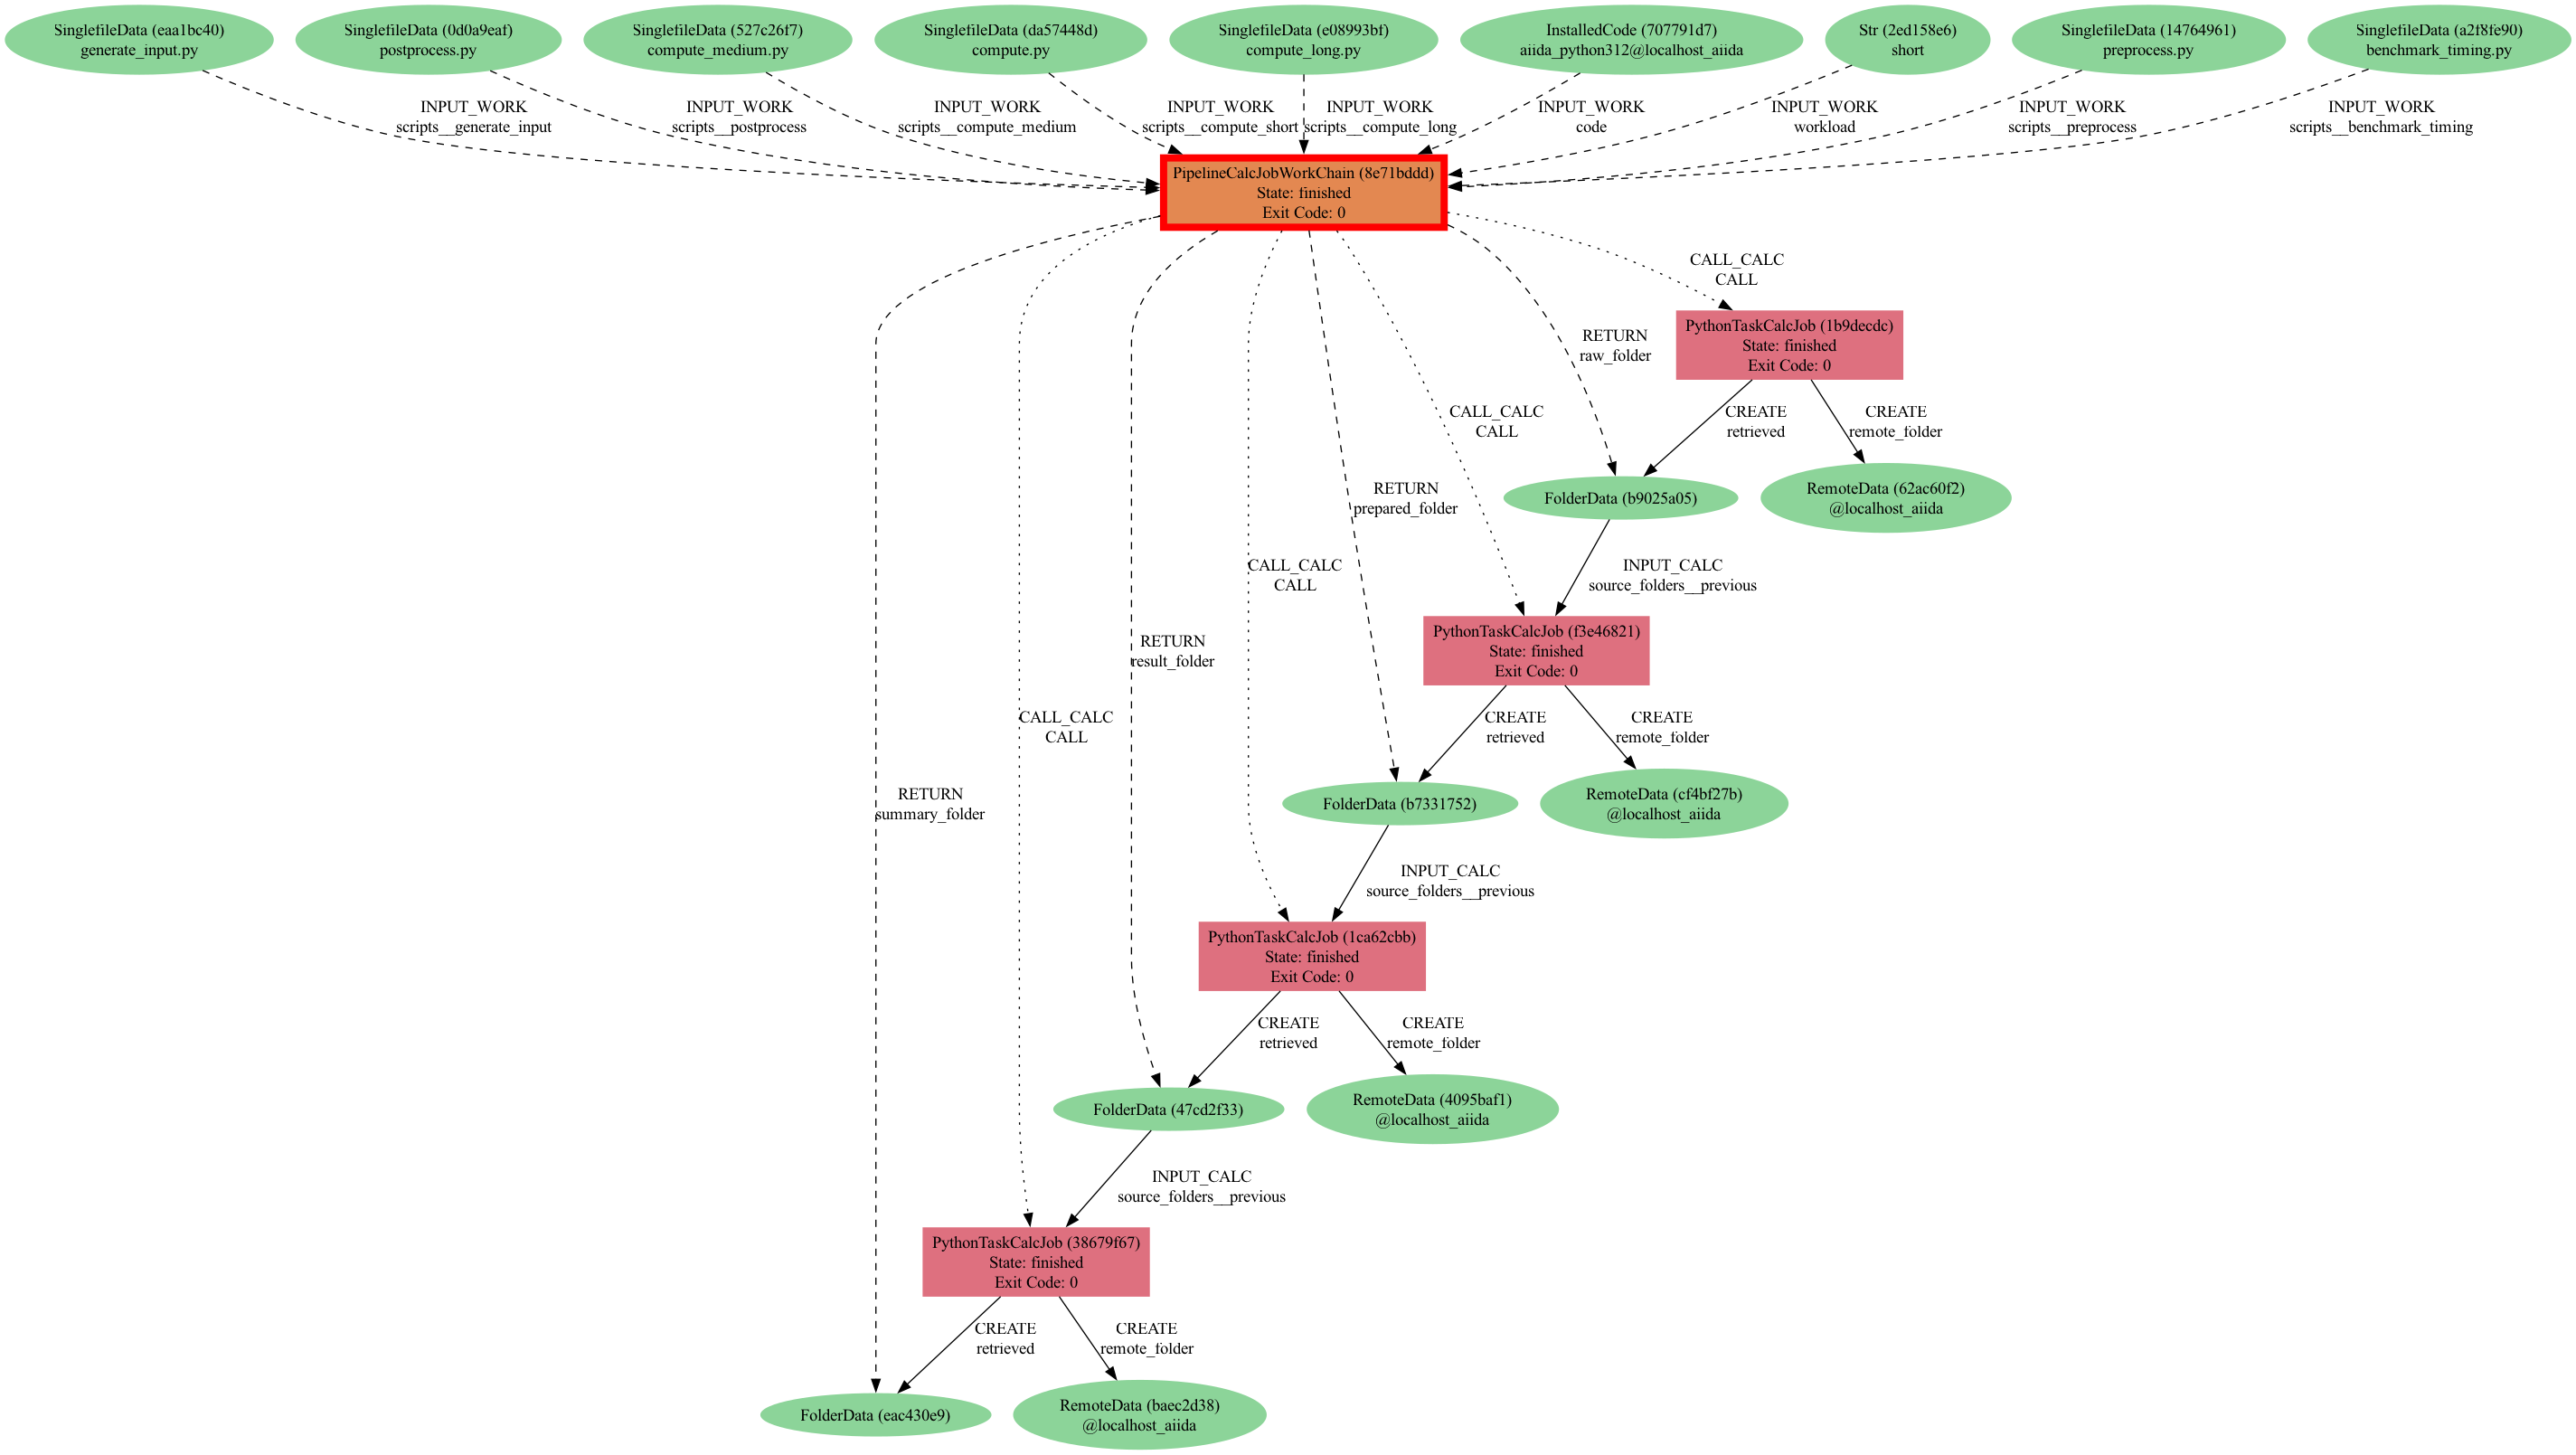
\includegraphics[width=\textwidth,height=0.40\textheight,keepaspectratio]{content/figs/aiida/aiida_pipeline_pk6147}
  \caption{Aus der AiiDA-Datenbank erzeugter Provenance-Graph des Pipeline-Laufs}
  \label{fig:ai:prov}
\end{figure}

\begin{figure}[H]
  \centering
  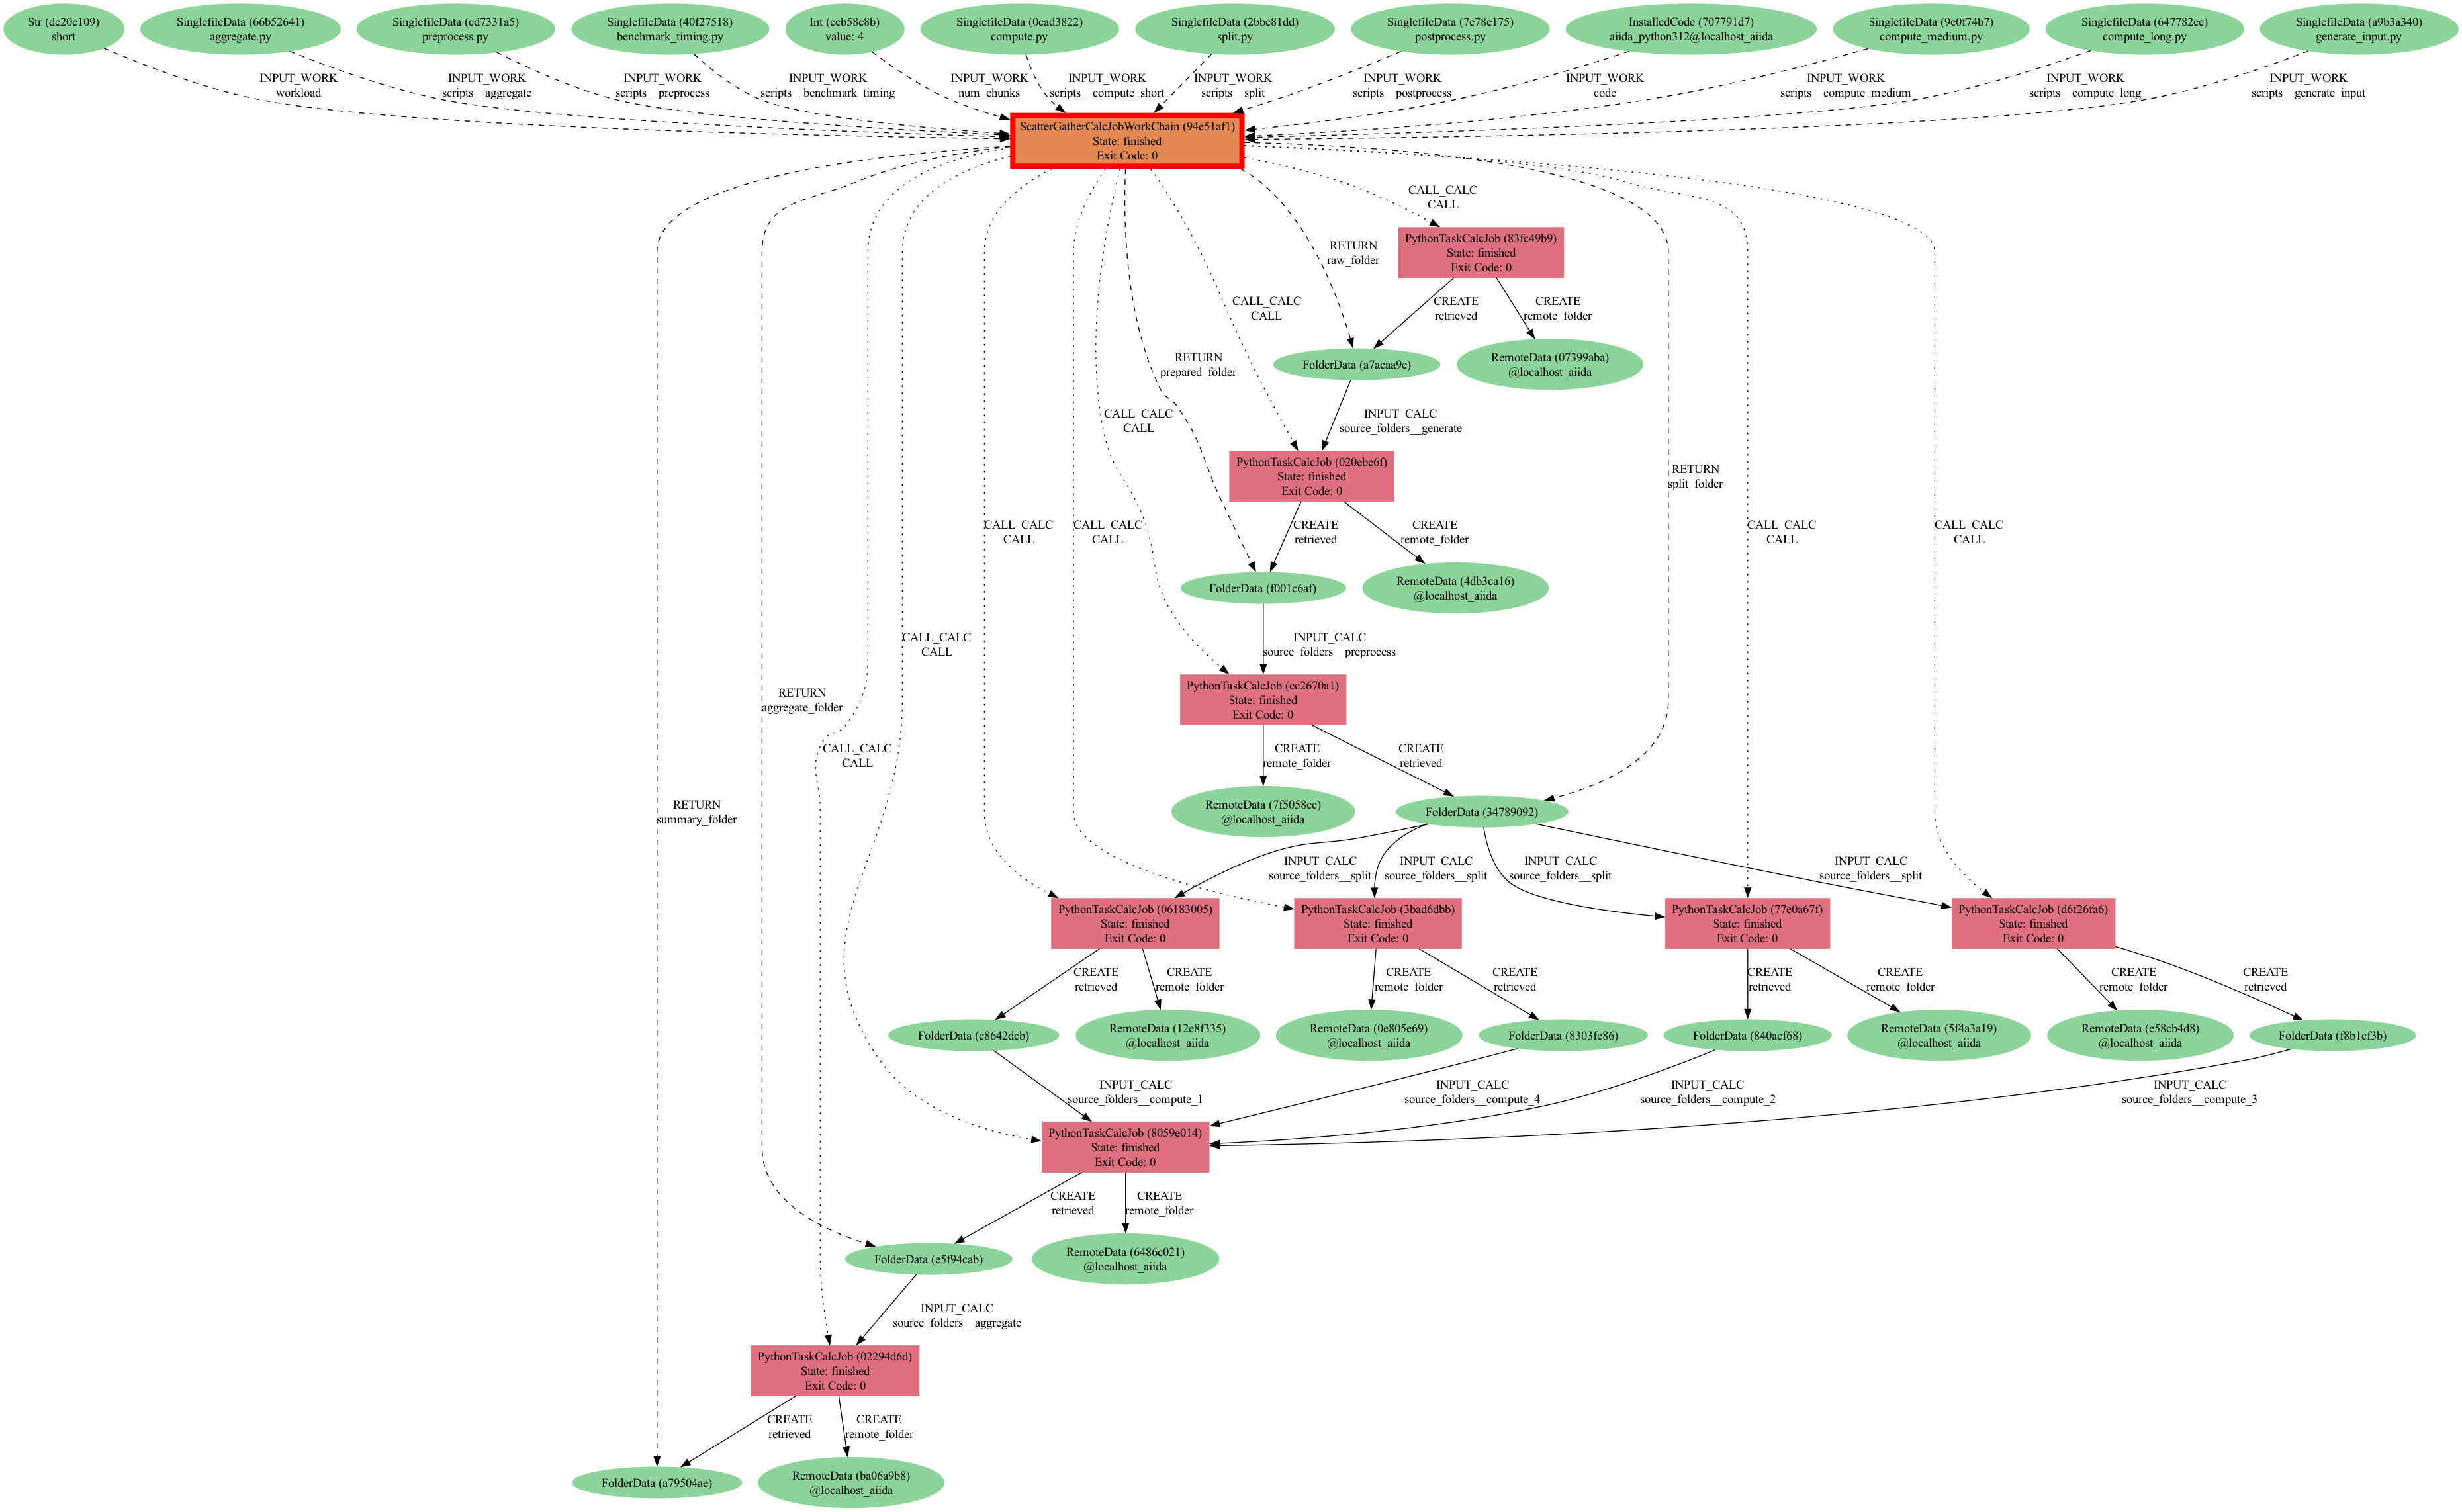
\includegraphics[width=\textwidth,height=0.40\textheight,keepaspectratio]{content/figs/aiida/scatter_gather_pk6182}
  \caption{Aus der AiiDA-Datenbank erzeugter Provenance-Graph eines Scatter-Gather-Laufs mit vier Teilstücken}
  \label{fig:ai:prov:sg}
\end{figure}